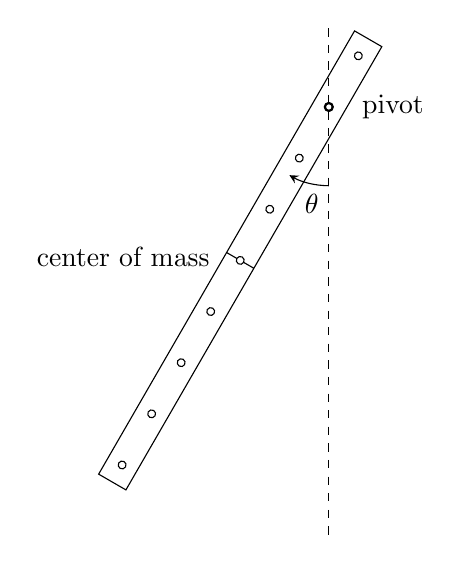
\begin{tikzpicture}

   \helpgrid{-4}{-6}{3}{2}      % Draw a grid to help place objects. Comment out in final version.
   
   \def\b{-5.5}         % Variable containing the position of the bottom of the bar
   \def\hw{0.2}         % Half-width of the bar
   \def\r{0.05}         % Radius of the pin-hole circles in the bar
   \def\cy{-2.25}       % Vertical position of center of bar

   \draw [dashed] (0,1) -- (0, \b);       % Dashed vertical line representing the equilibrium position. Note use of the variable \b

   \draw [rotate around={-30:(0,0)}]      % Rotate the following constructed object (bar with holes) about the origin by -30 degrees

      (-\hw, 1) rectangle (\hw, \b)       % The rectangle representing the outline of the order

      \foreach \y in {0.75,0,...,\b}      % We use a foreach loop to draw the circles on the bar placing them 0.75 units apart with one at the pivot
         {(0,\y) circle [radius=\r]}      % The foreach loop variable \y is used to position the center of the circles

      (-\hw, \cy) -- (-\r, \cy)       % Horizontal marker for Center of Mass which consists of lines on either side of the pin-hole (circle)
      (\r, \cy) -- (\hw, \cy)

      (-\hw-0.05, \cy-0.1) node[left] {center of mass}
   ;

   \draw [thick] (0,0) circle [radius=\r];          % Draw a thicker circle to represent the pivot

   % Show angle theta using an arc with an arrow
   \def\ar{1}         % Radius of arc used to define angle
   \draw [->,>=stealth] (0, -\ar) arc (-90:-120:\ar);           % Draw an arc with an arrow at the end for the angle
   \draw (-100:\ar+0.25) node {$\theta$};                       % Note the use of polar coordinates to place the variable theta

   \draw (\hw+0.1, 0) node[right] {pivot};

\end{tikzpicture}
